\clearpage

\lehead[]{\sf\hspace*{-2.00cm}\textcolor{white}{\colorbox{lightblue}{\parbox[c][0.70cm][b]{1.60cm}{
\makebox[1.60cm][r]{\thechapter}\\ \makebox[1.60cm][r]{ÜBUNG}}}}\hspace{0.17cm}\textcolor{lightblue}{\chaptertitle}}
\rohead[]{\textcolor{lightblue}{\chaptertitle}\sf\hspace*{0.17cm}\textcolor{white}{\colorbox{lightblue}{\parbox[c][0.70cm][b]{1.60cm}{\thechapter\\
ÜBUNG}}}\hspace{-2.00cm}}
%\chead[]{}
\rehead[]{\textcolor{lightblue}{AvHG, Inf, My}}
\lohead[]{\textcolor{lightblue}{AvHG, Inf, My}}

\section{Eigene Programme mit HJFrame -- Übungen}

\subsection{Aufgabe 1: Abstrakte Kunst}

Zeichne ein abstraktes Kunstwerk oder eine Figur. Teste dabei alle
vorgestellten Methoden der Klasse \myClass{Graphics} einmal aus. Verändere
außerdem die Schriftart sowie die Vorder- und Hintergrundfarbe des Programms.
Ändere auch die Größe des Anwendungsfensters.

\subsection{Aufgabe 2: Gespenster}

\begin{compactenum}[a)]
\item Erzeuge ein neues Anwendungsfenster mit einem schwarzen Hintergrund.
\item Programmiere eine Methode, die ein Gespenst an einer angegebenen Position
im Fenster zeichnet:
\begin{lstlisting}
public void gespenst(Graphics g, int x, int y)
\end{lstlisting}
Die Methode erhält das \myClass{Graphics}-Objekt („den Zeichenstift“) als
Parameter und die linke obere Ecke des Gespenstes, die in der Zeichnung mit
einem Kreuz markiert ist. Zeichne das Gespenst als ausgefüllten gelben Kreis.
Auf den Kreis werden die Augen und der Mund als ausgefüllte schwarze Ovale
aufgesetzt. Ein Kästchen in der Zeichnung entspricht einer Einheit von 10
Pixeln.

\begin{center}
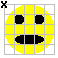
\includegraphics[width=0.2\textwidth]{./inf/SEKII/08_Java_Eigene_Programme_mit_HJFrame/Aufgabe2.png}
\end{center}

\item Rufe die Methode \lstinline|gespenst()| in der
\lstinline|myPaint()|-Methode mehrfach auf, so dass du Gespenster an
verschiedenen Positionen erhältst.
\end{compactenum}


\subsection{Aufgabe 3: Aufrufe von myPaint() zählen}

\begin{compactenum}[a)]
\item Schreibe ein Programm, das zählt wie oft die \lstinline|myPaint()|-Methode
aufgerufen wird. Der Zähler ist eine globale Integer-Variable, die zu Anfang
auf 0 gesetzt wird. Bei jedem Aufruf von \lstinline|myPaint()| wird der Zähler
um eins erhöht. Anschließend wird der Zähler mit der \myClass{Graphics}-Methode
\lstinline|drawString()| im Anwendungsfenster ausgegeben. Die Integer-Variable
wird dazu mit \lstinline|+| an einen String angehängt.
\item Teste aus, in welchen Situationen der Zähler erhöht wird. Verdecke dazu
vorübergehend das Programmfenster durch ein anderes Fenster oder verkleinere
das Fenster zu einem Icon.
\end{compactenum}


\subsection{Aufgabe 4: Quadrate zählen die Aufrufe von myPaint()}

Füge in das Programm aus Aufgabe 3 eine Zeile mit ausgefüllten grünen Quadraten
ein. Beim ersten Aufruf der \lstinline|myPaint()|-Methode wird nur ein Quadrat
gezeichnet, beim zweiten Aufruf werden zwei Quadrate gezeichnet, beim dritten
Aufruf drei Quadrate, usw.

Damit das Aussehen und die Position der Quadrate später leicht verändert werden
können, werden folgende Werte als Konstanten deklariert:

\begin{compactitem}
\item die Breite der Quadrate (Beispiel: \lstinline|final static int BREITE = 30;|)
\item der Abstand zwischen den Quadraten
\item die y-Position, an der die Quadrate beginnen
\item die x-Position, an der das erste Quadrat beginnt.
\end{compactitem} 

Programmiere die \lstinline|myPaint()|-Methode entsprechend. Verändere
anschließend das Aussehen der Quadrate, indem du die vier Konstanten
veränderst. Wenn dein Code sauber programmiert ist, muss nach der Änderung der
Konstanten ohne weitere Änderungen am Code noch alles funktionieren.


\subsection{Aufgabe 5: Gespenster-Dialog}

Im Programm soll eine Zeile mit lauter Gespenstern gezeichnet werden (benutze
dazu die Methode aus Aufgabe 2), zwischen denen jeweils 10 Pixel Abstand
liegen. Der Benutzer soll die Anzahl der Gespenster in einem Dialog eingeben.
Erzeuge den Dialog im Konstruktor des Programms und merke dir die vom Benutzer
eingegebene Zahl in einer globalen Variablen, die du in der
\lstinline|myPaint()|-Methode abfragst.

Was passiert, wenn man den Dialog in der \lstinline|myPaint()|-Methode erzeugt?


\subsection{Aufgabe 6: Ineinander geschachtelte Kreise}

Programmiere eine Methode, die die hier abgebildete Figur zeichnet: 

\begin{center}
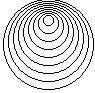
\includegraphics[width=0.2\textwidth]{./inf/SEKII/08_Java_Eigene_Programme_mit_HJFrame/Aufgabe6-1.png}
\end{center}

\begin{compactenum}[a)]
\item Die Methode erhält als Parameter das \myClass{Graphics}-Objekt, die
Zeichenfarbe und die linke obere Ecke der Figur (x- und y-Position). Alle anderen Werte wie
zum Beispiel die Breite dürfen in der Methode mit festen Zahlen eingestellt werden.
\item Stelle mit Hilfe der in a) programmierten Methode ein Bild aus mehreren
Figuren zusammen, die sich gegenseitig überlagern. Jede Figur hat eine eigene Farbe.
\item Programmiere eine Methode, die die hier abgebildete Figur zeichnet:

\begin{center}
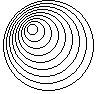
\includegraphics[width=0.2\textwidth]{./inf/SEKII/08_Java_Eigene_Programme_mit_HJFrame/Aufgabe6-2.png}
\end{center}

Die Methode erhält dieselben Parameter wie die Methode aus Aufgabe a). Erstelle
anschließend wieder ein Bild aus mehreren Figuren mit unterschiedlichen Farben,
die sich gegenseitig überlagern.
\item Programmiere eine Methode die, die die unten abgebildete Figur zeichnet.
Die Kreise werden bei dieser Figur nicht mehr hohl gezeichnet sondern mit zwei
sich abwechselnden Farben ausgefüllt. Beide Farben werden der Methode als
Parameter übergeben (zusätzlich zum \myClass{Graphics}-Objekt und der x- und y-
Position). Beachte, dass die Vordergrundfarbe vor jedem Malen eines Kreises mit
der Methode \lstinline|setColor()| gewechselt werden muss.

\begin{center}

\includegraphics[width=0.2\textwidth]{./inf/SEKII/08_Java_Eigene_Programme_mit_HJFrame/Aufgabe6-3.png}
\end{center}

Erstelle ein Bild aus mehreren Figuren mit unterschiedlichen Farben.
\end{compactenum}

\subsection{Aufgabe 7: Pyramide}

Programmiere ein Anwendungsfenster, das eine Pyramide aus Quadraten oder
Kreisen (Kreise erhalten exakt dieselben Parameter wie Quadrate) darstellt. Die
Breite der Quadrate soll im Code als Konstante vereinbart werden. Dadurch kann
man später leicht die Größe der Pyramide verändern, indem man einfach die
Konstante umsetzt. Außerdem werden der x- und der y-Wert der linken oberen Ecke
der Pyramide als Konstanten vereinbart und die Anzahl der Zeilen, die die
Pyramide haben soll. Wenn du die Lösung sauber programmiert hast, muss man
später ohne weitere Änderungen des Codes das Aussehen der Pyramide über die
Konstanten verändern können.

Tipp für die Programmierung: Zeichne die Pyramide zunächst auf Karo-Papier und
vergegenwärtige dir die Position der linken oberen Ecke der einzelnen Kästchen.

\begin{center}
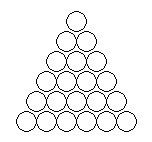
\includegraphics[width=0.3\textwidth]{./inf/SEKII/08_Java_Eigene_Programme_mit_HJFrame/Aufgabe7.png}
\end{center}


Erweiterung: Der Benutzer kann die Anzahl der Zeilen, die die Pyramide haben
soll, in einem Eingabe-Dialog eingeben. Die Pyramide wird je nach Eingabe des
Benutzer mit unterschiedlicher Größe gezeichnet.
